% !TEX TS-program = pdflatex
% !TEX encoding = UTF-8 Unicode

% This is a simple template for a LaTeX document using the "article" class.
% See "book", "report", "letter" for other types of document.

\documentclass[11pt]{article} % use larger type; default would be 10pt

\usepackage[utf8]{inputenc} % set input encoding (not needed with XeLaTeX)

%%% Examples of Article customizations
% These packages are optional, depending whether you want the features they provide.
% See the LaTeX Companion or other references for full information.

%%% PAGE DIMENSIONS
\usepackage{geometry} % to change the page dimensions
\geometry{a4paper} % or letterpaper (US) or a5paper or....
% \geometry{margin=2in} % for example, change the margins to 2 inches all round
% \geometry{landscape} % set up the page for landscape
%   read geometry.pdf for detailed page layout information

\setlength{\parindent}{0pt}
\setlength{\parskip}{\baselineskip}

\usepackage{caption}
\usepackage{hyperref}

\usepackage{graphicx} % support the \includegraphics command and options

% \usepackage[parfill]{parskip} % Activate to begin paragraphs with an empty line rather than an indent

%%% PACKAGES
\usepackage{array} % for better arrays (eg matrices) in maths
\usepackage{paralist} % very flexible & customisable lists (eg. enumerate/itemize, etc.)
\usepackage{verbatim} % adds environment for commenting out blocks of text & for better verbatim
\usepackage{subfig} % make it possible to include more than one captioned figure/table in a single float
\usepackage{natbib} % nice citations
% These packages are all incorporated in the memoir class to one degree or another...



%%% HEADERS & FOOTERS
\usepackage{fancyhdr} % This should be set AFTER setting up the page geometry
\pagestyle{fancy} % options: empty , plain , fancy
\renewcommand{\headrulewidth}{0pt} % customise the layout...
\lhead{}\chead{}\rhead{}
\lfoot{}\cfoot{\thepage}\rfoot{}

%%% SECTION TITLE APPEARANCE
\usepackage{sectsty}
\allsectionsfont{\sffamily\mdseries\upshape} % (See the fntguide.pdf for font help)
% (This matches ConTeXt defaults)

%%% ToC (table of contents) APPEARANCE
\usepackage[nottoc,notlof,notlot]{tocbibind} % Put the bibliography in the ToC
\usepackage[titles,subfigure]{tocloft} % Alter the style of the Table of Contents
\renewcommand{\cftsecfont}{\rmfamily\mdseries\upshape}
\renewcommand{\cftsecpagefont}{\rmfamily\mdseries\upshape} % No bold!

\usepackage{listings}
\usepackage{color}

\definecolor{dkgreen}{rgb}{0,0.6,0}
\definecolor{gray}{rgb}{0.5,0.5,0.5}
\definecolor{mauve}{rgb}{0.58,0,0.82}

\lstset{frame=tb,
  language=c,
  aboveskip=3mm,
  belowskip=3mm,
  showstringspaces=false,
  columns=flexible,
  basicstyle={\small\ttfamily},
  numbers=none,
  numberstyle=\tiny\color{gray},
  keywordstyle=\color{blue},
  commentstyle=\color{dkgreen},
  stringstyle=\color{mauve},
  breaklines=true,
  breakatwhitespace=true,
  tabsize=3
}

%%% END Article customizations

%%% The "real" document content comes below...

\title{Procedurally grown trees}
\author{Andreas Valter}
%\date{} % Activate to display a given date or no date (if empty),
         % otherwise the current date is printed

\begin{document}
\maketitle
\begin{figure}[htp]
	\centering
	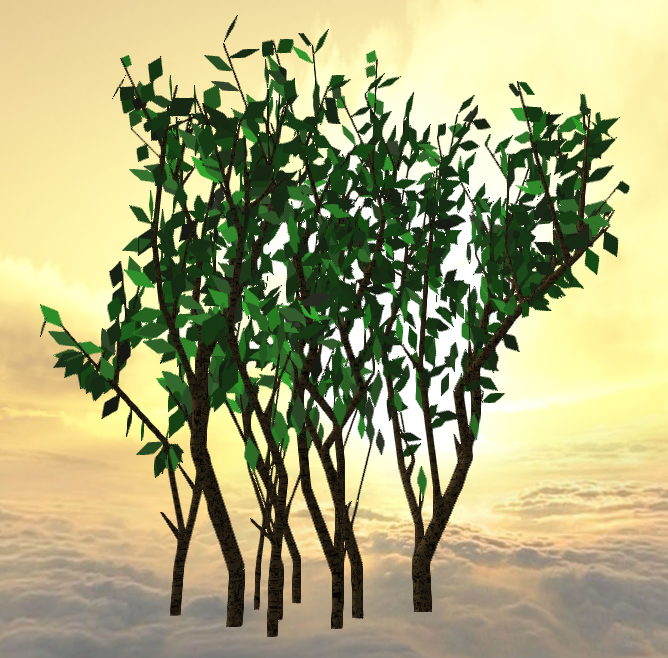
\includegraphics[width=0.4\textwidth]{manytree.png}
	%\caption{A bunch of trees generated with the algorithm described in this report.}
	\label{fig:asd}
\end{figure}

\section{Background}
When modelling the growth of trees, their growth follows a specific procedure that can be modelled.
The system is called a fractal and is a natural phenomenon where the same pattern repeats itself at different scales.
The smallest branch of a tree looks like a tree itself.
But even if a tree follows these rules, it will also take other things, like the amount of sun the leaves can absorb, water supply into consideration when deciding the fate of each branch and the whole tree.
This makes it so that when observing a real tree, the features of a fractal pattern is somewhat visible but it is hidden behind the fate of the tree as it has grown.
If these are taken into consideration when creating the fractal pattern of the tree, it will look close to a real tree.

When simulating the growth of a tree, it is important to define a couple terms that helps when describing the different steps of the growth procedure.
The point where leafs are attached to a stem are called \emph{nodes}.
The part of the stem between two nodes are called an \emph{inter-node}.
An inter-node, connected leafs and bud is a \emph{metamer}.
\cite{Palubicki:2009:STM:1531326.1531364}

\section{Implementation}
The implementation follows the report by Pablucki et al. \cite{Palubicki:2009:STM:1531326.1531364} that describes a method for creating self-organizing trees.
It describes a general outline of the method they present, as well as several alternatives for the steps that makes up for the total algorithm.
Due to time constraints, all of the described methods has not been implemented in this report.
This report describes the implementation of said algorithms together with some extensions that were made to generate and render the trees with interactive framerates.

\subsection{Tree generation}
The tree is generated on the CPU using a multithreaded approach in critical parts of the implementation.
Growth is handled in several steps that uses the environment together with existing buds to determine the state of the tree after the current growth cycle.
This allows for a dynamic and procedural growth producing unique trees over time.

\subsubsection{Environmental input}
The presented method starts with environmental input where the environment around each existing bud is examined to determine the state for those parts of the tree.
Palubicki et al.\cite{Palubicki:2009:STM:1531326.1531364} presents two different techniques for handling the availability of growth in space around the tree and the optimal growth direction for branches.
One is called space colonization and the other is called shadow propagation.

Space colonization uses a uniform distribution of points in the world, each bud has an occupancy zone as well as a perception volume.
When evaluating available space, available points within the perception volume are found.
By summarizing the direction towards each of them, a optimal growth direction is found.
When adding new points, the points within the occupancy zone are consumed.
A binary shadow value is also provided that is zero when no points are available and one when points were found.

Shadow propagation uses a voxel grid to keep track of the environment around each bud.
Each newly formed bud adds a shadow value to the voxel grid in a pyramid below it with a shadow value that propagates to the voxels underneath.
This imitates a prenumbra shadow from each bud and as the shadow value increases, the probability for growth towards that specific voxel decreases.
Optimal directions are calculated by finding the gradient of the shadow grid in the bud point to make it grow towards the direction where there is the most light.
When bud points are not contained within the grid, the size of the grid is doubled in that direction until the resized grid covers the point.
The data from the previous grid are copied into the resized grid together with the data from the new bud point.\cite{Palubicki:2009:STM:1531326.1531364}

\subsubsection{Bud fate}
The technique that were implemented is an extension to the Borchet-Honda model that is described by Palubicki et al.\cite{Palubicki:2009:STM:1531326.1531364}
The bud fate is decided using the shadow value retrieved from the environmental input calculation for each bud.
This value is then distributed towards the light accumalative producing the total light reached to each branch and its child branches.

The number of metamers produced by the bud is calculated as the light value floored and the length of the branch is the light value divided by the number of metamers.

\subsubsection{Shoots creation}
The bud fate decides what shoots to add and their length.
Metamers are added in an iterative fashion to the branches represented as a binary tree.
Each branch has two childs, the terminal and the lateral branch.\cite{Palubicki:2009:STM:1531326.1531364}

\subsubsection{Branch width}
The branch width is calculated by adding width back towards the root from the end branches of the tree.
Each leaf adds a starting width that is accummulated back to the root as the tree grows.
This requires that shred branches are stored so that the width of the tree does not change in width as branches are removed.\cite{Palubicki:2009:STM:1531326.1531364}

\subsection{Rendering}
To be able to visualize the tree and to produce an output as quickly as possible, shaders were used to produce a model.
As the tree are done calculating the new state, the collection of branches are sent to the renderer.
After finishing computing the new branches after a production cycle, the tree data is uploaded to the GPU in a buffer of packed data.
The data is uploaded per branch and consists of start and end positions and the width at each of the joints.
A compute shader is responsible for converting the input data into a mesh with texture coordinates, positions and normals.

\begin{equation}
	\label{eq:DelAlpha}
	\Delta \alpha = \frac{2 \pi}{N_{e}}
\end{equation}
\begin{equation}
	\label{eq:vdir}
	v_{dir} = b_{s} - b_{e} 
\end{equation}
\begin{equation}
	\label{eq:vcross}
	v_{orth2} = v_{dir}\times v_{orth1}
\end{equation}
\begin{equation}
	\label{eq:alphai}
	\alpha_{i} = \sum_{j = 0}^{i}\Delta \alpha
\end{equation}
\begin{equation}
	\label{eq:betai}
	N_{i} = sin(\alpha_{i}) \hat{v}_{orth2} + cos(\alpha_{i}) \hat{v}_{orth1}
\end{equation}
\begin{equation}
	\label{eq:pi}
	p_{i}=p_{c} +  \hat{N}_{i} w_{c}
\end{equation}

The number of faces on each branch is decided by an uniform value $N_{e}$.
This value is used to divide the angular space around the branch into segments to be represented with faces.
The angular space $ \Delta \alpha $ that each face represents is calculated with equation \ref{eq:DelAlpha}.
The branch direction $ v_{dir} $ is the difference between the branch start position $ b_{s} $
and the branch end position $ b_{e} $ calculated in equation \ref{eq:vdir}.
The first orthogonal vector $ v_{orth1} $ is calculated by flipping the parameters of the direction vector.

\begin{lstlisting}
vec3 orthogonal(in vec3 dir)
{
	return abs(dir.x) > abs(dir.z) ? 
		vec3(-dir.y, dir.x, 0.0) : vec3(0.0, -dir.z, dir.y);
}
\end{lstlisting}

\begin{figure}[htp]
	\centering
	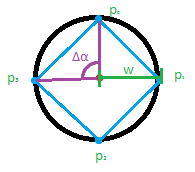
\includegraphics[width=0.4\textwidth]{branchAngles.png}
	\caption{Crossection of tree branch visualized with four edges.}
	\label{fig:branchAngles}
\end{figure}

As is shown in equation \ref{eq:vcross}, crossing the branch direction vector $ v_{dir} $ and the orthogonal vector $ v_{orth1} $ results in the second orthogonal vector $ v_{orth2} $.
$ v_{orth1} $ and $ v_{orth2} $ is used as corners of a unit circle and the local position in unit space which is also the normal $ N_{i} $ is calculated using the current angle $ \alpha_{i} $ calculated as a sum of $ \Delta \alpha $ in equation \ref{eq:alphai} in a sin and a cosine term multiplied with normalized versions of the two orthogonal vectors.
By multiplying with the branch width at the current edge of the branch $ w_{c} $ and adding the position on the branch $ p_{c} $, the position of the bark surface $ p_{i} $ is achieved.
This is visualized in \autoref{fig:branchAngles} that shows an example using four edges to represent the tree branch.
The resulting geometry is shown in blue.


The normal vector $ N_{i} $ is also stored at each of the edges.
An index buffer is also used to omit some duplicate data per face and convert the vertex data that is stored per quad into triangles that can be used to render.

Texture coordinates are calculated using two different levels of detail depending on the mean width of the current face of the branch.
These levels of detail are stored in the same texture and to give each face a separate set of texture coordinates depending on what LOD they are assigned, two atomic counters are used.

Atomic counters are integer objects that can be used to get unique ids in a multi thread environment.
Each fragment can retrieve a ID from the counters that can be converted to a spot within the texture.
The texture is built up with a upper half responsible for storing lower levels of detail and the lower part for higher levels of detail.
The size of each texture segment is divided by four in the lower LOD compared to the size of the higher LOD.
This makes it possible to have unique textures for each branch and describe the whole tree using a reasonably sized texture.

The computed tree branches are then used to generate the texture map and a second shader pair consisting of a vertex shader and a fragment shader.
The vertex shader outputs the texture coordinates as positions which generates fragments for the texture of each tree branch.
World positions are also sent to the compute shader to use in the noise functions that creates the diffuse, normal and displacement map of the tree bark.

The tree is rendered using a tessellation shader that use the displacement map to offset the generated vertices to their correct location.
The result is then drawn to the GBuffer using the diffuse and the normal texture to produce the final output.

Leafs are also generated using a compute shader but updated each frame.
Each leaf consists of two triangles creating a parallelogram with one of the edges in origo.
The direction of the leaf is decided by the bud direction together with a noise term that changes over time with different noise functions in each component of the vector.
The edges of the parallelogram is calculated by finding an orthogonal vector to the bud direction and placing those positions a bit away from the leaf position, with a small offset in the orthogonal direction and the negative orthogonal direction.

The color of the leafs are green with a small randomized offset between leafs in the green channel in the rgb to add some complexity to the leafs.
Normals are calculated by crossing the leaf direction with the first orthogonal vector. To make sure that the leafs are animated, the leaf calculation is made each frame.

\begin{figure}[htp]
	\centering
	
\includegraphics[width=0.4\textwidth]{1tree.png}
	\caption{Single grown tree using the extended BH bud fate model.}
	\label{fig:res_1tree}
\end{figure}

\section{Results}
When running the application, the growth of the tree is displayed in the application view port.
As the tree grows, leafs are dynamically added and moves as touched by a breeze.
\autoref{fig:res_1tree} shows a screen capture of a single tree grown over 20 growth cycles.

The textures are without seams in both joints and between segments of the same branch.
This is visible in \autoref{fig:closeup} where the tree are dividing into several branches.
\autoref{fig:joints} shows the two LODs in action.

\begin{figure}[htp]
	\centering
	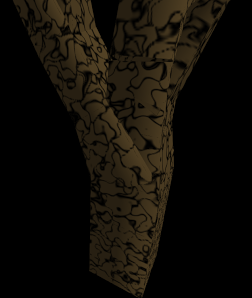
\includegraphics[width=0.4\textwidth]{joints.png}
	\caption{Close up showing texture adopting over tree branches.}
	\label{fig:closeup}
\end{figure}

\begin{figure}[htp]
	\centering
	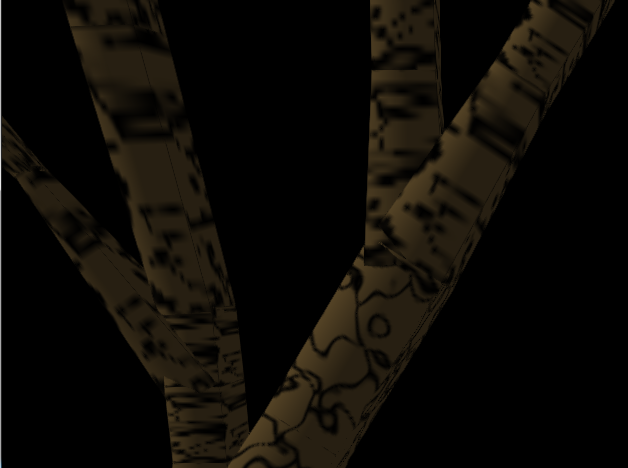
\includegraphics[width=0.4\textwidth]{closeup.png}
	\caption{Showing both LODs operating on two different branches.}
	\label{fig:joints}
\end{figure}

The total time to grow the tree was 138ms and most of that time was spent adding points to the voxel grid.
This is visualized in \autoref{fig:res_timingTotal} where the total time per growth cycle is shown and divided into the required steps performed when generating the tree.

\begin{figure}[htp]
	\centering
	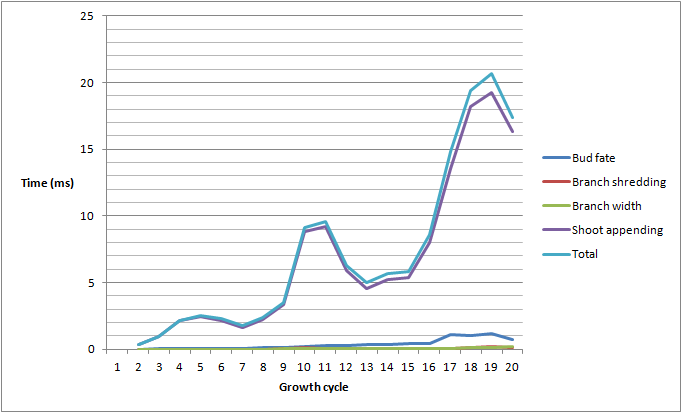
\includegraphics[width=0.8\textwidth]{timingTotal.png}
	\caption{Total simulation time per growth stage for a tree.}
	\label{fig:res_timingTotal}
\end{figure}

The generated branch faces does not take the angle compared to parent and child branches which leads to holes in the mesh as is seen in \autoref{fig:res_treehole}.

\begin{figure}[htp]
	\centering
	
\includegraphics[width=0.4\textwidth]{treehole.png}
	\caption{Problems in tree branch generation.}
	\label{fig:res_treehole}
\end{figure}

\begin{figure}[!htp]
	\centering
	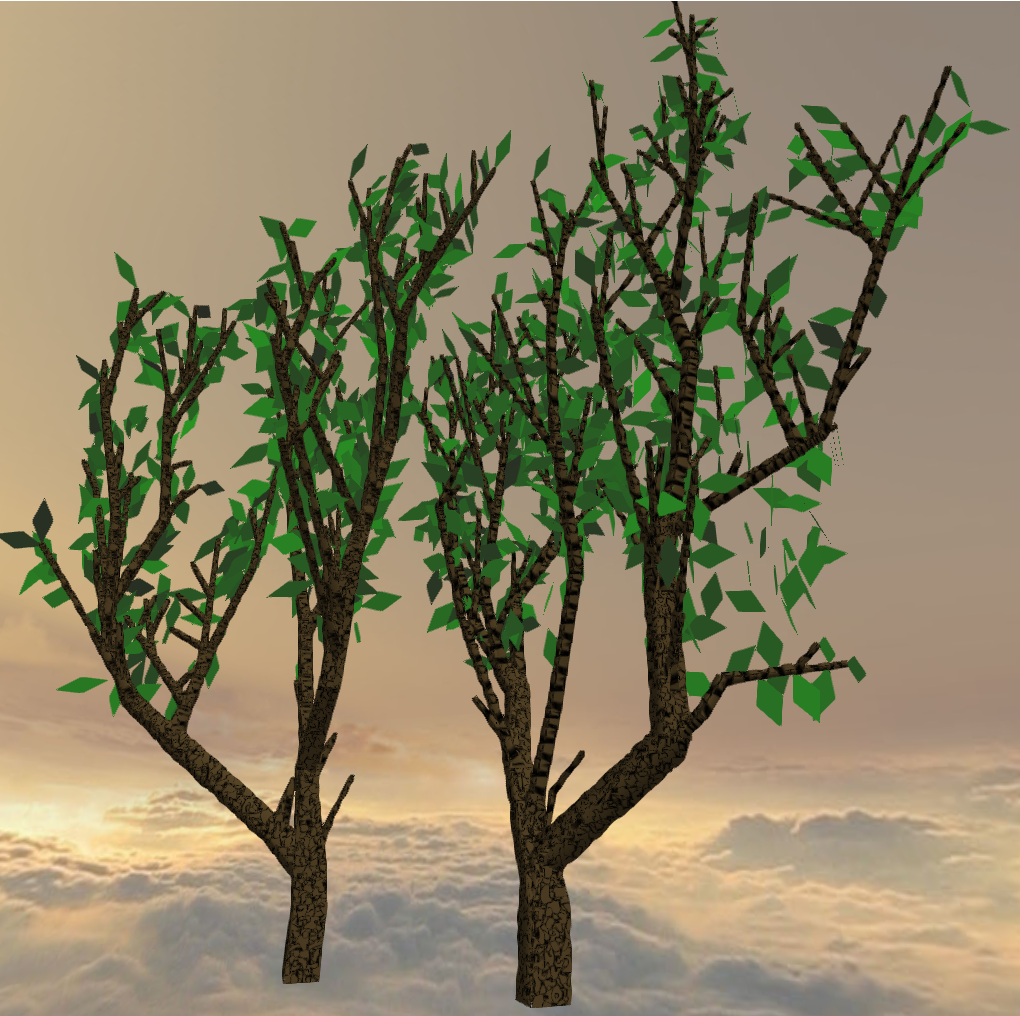
\includegraphics[width=0.4\textwidth]{2tree.png}
	\caption{Two grown tree using the extended BH bud fate model.}
	\label{fig:res_2tree}
\end{figure}

\autoref{fig:res_2tree} shows the same algorithm operating on two trees growing at the same time sharing grid.



\section{Conclusions}
The tree structure is thicker at the top part of the tree because of the shadow grid that shreds branches that shadowed by overlying branches.
That the extended BH model makes it almost impossible to create a main terminal branch in the tree pointing upwards.
This results in a lot wider trees that always has a branch at the begining.
By implementing the pirority bud fate model, the main branch could be prioritized, resulting in a tree more distinct tree shape with a thick terminal branch and smaller branches pointing out from it.

As can be seen in \autoref{fig:res_2tree}, the algorithm succesfully handles dynamic growth of several trees that interact with each other without intersections.

The speed of the tree generation could be increased using a octree structure for handling the grid, this would make it faster to increase the size of the grid while keeping the size of the grid smaller because it is a sparse structure that only keeps data for filled voxels.
And just as it is for real trees, computer generated trees are mostly air or empty voxels.

The quality of the textures could be increased by using a set of generated 2d textures for each branch and interpolate them between branches using weights in the joints.
Using several lods for the textures makes it possible to have a high quality of each tree while keeping them unique.
But they suffer from running out of texture space when the tree grows big enough.
At the same time each tree could generate their own set of base textures that are randomly used between tree branches of the same tree.
This would result in unique trees that still keep the detail at a high level.

More work has to be made to make sure that branches are kept connected as their width increases.
As it is now, when two branches with a large angular difference are rendered, a hole is noticeable in the seam.
This could be resolved using the angle between the two branches when calculating branch face positions to take this fact into consideration.
A simple method could be to apply a scaled offset in the direction of the branch depending on the width of the branch but this could either introduce artefacts where branches intersect too much or still leave a gap.
One way to achieve the correct result is to calculate the face edges once for each joint between two branches.
The simplest method would be to use the same algorithm as is currently used but for each joint instead of each branch and write this to the vertex buffer and use the index buffer to correctly index into the vertex buffer.
The only problem this would cause is that this would not make the current texture system work because it requires each face to have its own texture coordinates.

Because shred branch positions are kept it would be possible to add textures for shredded branches showing the interior of the tree to visualize that shredding has occured.

After looking at the results, the generated trees achieves a decent level of detail and realism while working in real time with fast threaded generation.

\bibliographystyle{abbrv}
\bibliography{report}

\end{document}
